%%%%%%%%%%%%%%%%%%%%%%%%%%%%%%%%%%%%%%%%%%%%%%%%%%%%%%%%%%%%%%%%%%%%%%%%%%%%%%%%
%% Plantilla de memoria en LaTeX para la EIF - Universidad Rey Juan Carlos
%%
%% Por Gregorio Robles <grex arroba gsyc.urjc.es>
%%     Grupo de Sistemas y Comunicaciones
%%     Escuela de Ingeniería de Fuenlabrada
%%     Universidad Rey Juan Carlos
%% (muchas ideas tomadas de Internet, colegas del GSyC, antiguos alumnos...
%%  etc. Muchas gracias a todos)
%%
%% La última versión de esta plantilla está siempre disponible en:
%%     https://github.com/gregoriorobles/plantilla-memoria
%%
%% Para obtener PDF, ejecuta en la shell:
%%   make
%% (las imágenes deben ir en PNG o JPG)

%%%%%%%%%%%%%%%%%%%%%%%%%%%%%%%%%%%%%%%%%%%%%%%%%%%%%%%%%%%%%%%%%%%%%%%%%%%%%%%%

\documentclass[a4paper, 12pt]{book}
%\usepackage[T1]{fontenc}

\usepackage[a4paper, left=2.5cm, right=2.5cm, top=3cm, bottom=3cm]{geometry}
\usepackage{times}
\usepackage[utf8]{inputenc}
\usepackage[spanish]{babel} % Comenta esta línea si tu memoria es en inglés
\usepackage{url}
%\usepackage[dvipdfm]{graphicx}
\usepackage{graphicx}
\usepackage{float}  %% H para posicionar figuras
\usepackage[nottoc, notlot, notlof, notindex]{tocbibind} %% Opciones de índice
\usepackage{latexsym}  %% Logo LaTeX

% Escribe el título y el nombre del autor / autora para que se use bien
% en otras partes de la plantilla
% Dependiendo de las partes de la plantilla, a veces aparecerán tal
% cual los escribas, a veces totalmente en mayúsculas, a veces de otras
% formas
\title{Mapas de Terreno para Realidad Virtual}
\author{José Fuhui Pérez Contreras}

% Guarda el título, el autor y la fecha en variables
\makeatletter
\let\thetitle\@title
\let\theauthor\@author
\let\thedate\@date
\makeatother

\renewcommand{\baselinestretch}{1.5}  %% Interlineado

\begin{document}

\renewcommand{\refname}{Bibliografía}  %% Renombrando
\renewcommand{\appendixname}{Apéndice}


%%%%%%%%%%%%%%%%%%%%%%%%%%%%%%%%%%%%%%%%%%%%%%%%%%%%%%%%%%%%%%%%%%%%%%%%%%%%%%%%
% PORTADA

\begin{titlepage}
\begin{center}
\includegraphics[scale=0.6]{img/URJ_logo_Color_POS.png}

\vspace{1.75cm}

\LARGE
ESCUELA DE INGENIERÍA DE FUENLABRADA
\vspace{1cm}

\LARGE
GRADO EN INGENIERÍA TELEMÁTICA

\vspace{1cm}
\LARGE
\textbf{TRABAJO FIN DE GRADO}

\vspace{2cm}

\Large
\MakeUppercase{\thetitle}

\vspace{2cm}

\large
Autor : \theauthor \\
Tutor : Dr. David Moreno Lumbreras\\
\vspace{1cm}

\large
Curso académico 2024/2025

\end{center}
\end{titlepage}

\newpage
\mbox{}
\thispagestyle{empty} % para que no se numere esta pagina



%%%%%%%%%%%%%%%%%%%%%%%%%%%%%%%%%%%%%%%%%%%%%%%%%%%%%%%%%%%%%%%%%%%%%%%%%%%%%%%%
%%%% Licencia
\clearpage
\pagenumbering{gobble}
\chapter*{}

\vspace{12cm}

%% Licencia de publicación en abierto elegida
%% Ver detalles en https://ofilibre.urjc.es/guias/tfg-abierto/

\begin{flushright}
\includegraphics[scale=0.6]{img/by-sa}
%\includegraphics[scale=0.6]{img/by}

%% Poner el año adecuado
\noindent©2025 \theauthor  \\
Algunos derechos reservados  \\
Este documento se distribuye bajo la licencia \\
``Atribución-CompartirIgual 4.0 Internacional'' de Creative Commons, \\
disponible en \\
\url{https://creativecommons.org/licenses/by-sa/4.0/deed.es}
\end{flushright}

%%%%%%%%%%%%%%%%%%%%%%%%%%%%%%%%%%%%%%%%%%%%%%%%%%%%%%%%%%%%%%%%%%%%%%%%%%%%%%%%
%%%% Dedicatoria

\chapter*{}
\pagenumbering{Roman} % para comenzar la numeracion de paginas en numeros romanos
\begin{flushright}
\textit{Dedicado a \\
mis padres}
\end{flushright}

%%%%%%%%%%%%%%%%%%%%%%%%%%%%%%%%%%%%%%%%%%%%%%%%%%%%%%%%%%%%%%%%%%%%%%%%%%%%%%%%
%%%% Agradecimientos

\chapter*{Agradecimientos}
%\addcontentsline{toc}{chapter}{Agradecimientos} % si queremos que aparezca en el índice
\markboth{AGRADECIMIENTOS}{AGRADECIMIENTOS} % encabezado 

Quiero agradecer a todas las personas que me han ayudado a lo largo de mi carrera, y en especial a mis amigos de clase
y a mi tutor, David, por su apoyo y ayuda en la realización de este trabajo. También quiero agradecer a mis padres por su apoyo incondicional 
y por haberme dado la oportunidad de estudiar en esta universidad.

%%%%%%%%%%%%%%%%%%%%%%%%%%%%%%%%%%%%%%%%%%%%%%%%%%%%%%%%%%%%%%%%%%%%%%%%%%%%%%%%
%%%% Resumen

\chapter*{Resumen}
%\addcontentsline{toc}{chapter}{Resumen} % si queremos que aparezca en el índice
\markboth{RESUMEN}{RESUMEN} % encabezado

Este proyecto tiene como objetivo la creación de un componente en tres dimensiones compatible
con la realidad virtual. El componente utiliza \textit{APIS} de \textit{Mapbox} y \textit{OpenStreetMap} 
para la creación de mapas de terreno en tres dimensiones. Se pretende que el componente
pueda ser utilizado en aplicaciones de realidad virtual y que sea fácil de integrar
en otros proyectos.

El componente se ha desarrollado utilizando \textit{JavaScript} y \textit{HTML}, apoyándose en
los entornos de trabajo de \textit{Node.js}, \textit{A-Frame} (y, por tanto, \textit{WebGL} y \textit{Three.js}) y \textit{BabiaXR}.
La intención es que esté disponible en la web para que cualquier persona pueda
utilizarlo y contribuir a su desarrollo.

Los mapas son una herramienta muy útil para la visualización de datos y la
navegación en entornos tridimensionales. Durante toda la historia se han valorado
los mapas como una herramienta fundamental para la exploración y el
conocimiento del mundo. En la actualidad, con el auge de la realidad virtual y la
realidad aumentada, los mapas han cobrado una nueva dimensión y se están convirtiendo
en una herramienta esencial para la creación de experiencias inmersivas. Es por
ello que pienso que este proyecto es relevante y puede tener un impacto
significativo en el campo de la realidad virtual y la visualización de datos.

% \begin{itemize}
%   \item ¿De qué va este proyecto? ¿Cuál es su objetivo principal?
%   \item ¿Cómo se ha realizado? ¿Qué tecnologías están involucradas?
%   \item ¿En qué contexto se ha realizado el proyecto? ¿Es un proyecto dentro de un marco general?
% \end{itemize}

% Lo mejor es escribir el resumen al final.

%%%%%%%%%%%%%%%%%%%%%%%%%%%%%%%%%%%%%%%%%%%%%%%%%%%%%%%%%%%%%%%%%%%%%%%%%%%%%%%%
%%%% Resumen en inglés

\chapter*{Summary}
%\addcontentsline{toc}{chapter}{Summary} % si queremos que aparezca en el índice
\markboth{SUMMARY}{SUMMARY} % encabezado

This project aims to create a three-dimensional component compatible
with virtual reality. The component uses APIs from \textit{Mapbox} and \textit{OpenStreetMap} 
to generate three-dimensional terrain maps. The goal is for the component
to be usable in virtual reality applications and to be easy to integrate
into other projects.

The component has been developed using \textit{JavaScript} and \textit{HTML}, relying on
the \textit{Node.js}, \textit{A-Frame} (and therefore \textit{WebGL} and \textit{Three.js}) and \textit{BabiaXR}
frameworks. The intention is to make it available on the web so that anyone can
use it and contribute to its development.

Maps are a very useful tool for data visualization and
navigation in three-dimensional environments. Throughout history, maps have been valued
as a fundamental tool for exploration and
understanding of the world. Nowadays, with the rise of virtual reality and
augmented reality, maps have taken on a new dimension and are becoming
an essential tool for creating immersive experiences. That is
why I believe this project is relevant and may have a significant impact
in the field of virtual reality and data visualization.


%%%%%%%%%%%%%%%%%%%%%%%%%%%%%%%%%%%%%%%%%%%%%%%%%%%%%%%%%%%%%%%%%%%%%%%%%%%%%%%%
%%%%%%%%%%%%%%%%%%%%%%%%%%%%%%%%%%%%%%%%%%%%%%%%%%%%%%%%%%%%%%%%%%%%%%%%%%%%%%%%
% ÍNDICES %
%%%%%%%%%%%%%%%%%%%%%%%%%%%%%%%%%%%%%%%%%%%%%%%%%%%%%%%%%%%%%%%%%%%%%%%%%%%%%%%%

% Las buenas noticias es que los índices se generan automáticamente.
% Lo único que tienes que hacer es elegir cuáles quieren que se generen,
% y comentar/descomentar esa instrucción de LaTeX.

%%%% Índice de contenidos
\tableofcontents 
%%%% Índice de figuras
\cleardoublepage
%\addcontentsline{toc}{chapter}{Lista de figuras} % para que aparezca en el indice de contenidos
\listoffigures % indice de figuras
%%%% Índice de tablas
%\cleardoublepage
%\addcontentsline{toc}{chapter}{Lista de tablas} % para que aparezca en el indice de contenidos
%\listoftables % indice de tablas


%%%%%%%%%%%%%%%%%%%%%%%%%%%%%%%%%%%%%%%%%%%%%%%%%%%%%%%%%%%%%%%%%%%%%%%%%%%%%%%%
%%%%%%%%%%%%%%%%%%%%%%%%%%%%%%%%%%%%%%%%%%%%%%%%%%%%%%%%%%%%%%%%%%%%%%%%%%%%%%%%
% INTRODUCCIÓN %
%%%%%%%%%%%%%%%%%%%%%%%%%%%%%%%%%%%%%%%%%%%%%%%%%%%%%%%%%%%%%%%%%%%%%%%%%%%%%%%%

\cleardoublepage
\chapter{Introducción}
\label{sec:intro} % etiqueta para poder referenciar luego en el texto con ~\ref{sec:intro}
\pagenumbering{arabic} % para empezar la numeración de página con números

% En este capítulo se introduce el proyecto.
% Debería tener información general sobre el mismo, dando la información sobre el contexto en el que se ha desarrollado.

% No te olvides de echarle un ojo a la página con los cinco errores de escritura más frecuentes\footnote{\url{http://www.tallerdeescritores.com/errores-de-escritura-frecuentes}}.

% Aconsejo a todo el mundo que mire y se inspire en memorias pasadas.
% Las memorias de los proyectos que he llevado yo están (casi) todas almacenadas en mi web del GSyC\footnote{\url{https://gsyc.urjc.es/~grex/pfcs/}}.

% En mayo de 2023 me apunté a un curso de innovación docente donde nos pidieron hacer un podcast con temática docente. Aproveché entonces para hacer un podcast de unos 30 minutos donde en los primeros quince minutos introducía LaTeX y la memoria, y en los segundos hacía hincapién en aquellas cosas que más os cuestan utilizar en la memoria: las figuras, las tablas y las citas. Podéis escuchar el podcast en Internet\footnote{\url{https://podcasters.spotify.com/pod/show/gregorio-robles9/episodes/Tu-memoria-de-Trabajo-Fin-de-Grado-o-de-Mster-en-LaTeX-e23hucr/a-a58kp2}}.

En los últimos años, el desarrollo de tecnologías inmersivas como la realidad virtual (VR) y la realidad aumentada (AR) ha propiciado nuevas formas de interactuar con la información digital. En este contexto, los mapas tridimensionales se presentan como una herramienta clave para enriquecer experiencias inmersivas, facilitar la navegación en entornos complejos y mejorar la visualización de datos geoespaciales. Este proyecto se enmarca en dicha línea de innovación, proponiendo la creación de un componente web en tres dimensiones que permita representar mapas de terreno realistas y compatibles con dispositivos de realidad virtual.

El componente desarrollado hace uso de diversas tecnologías modernas del ecosistema web, como \textit{A-Frame}, \textit{WebGL} y \textit{Three.js}, facilitando la creación de entornos 3D interactivos en navegadores estándar. A su vez, se apoya en servicios de terceros como \textit{Mapbox} y \textit{OpenStreetMap}, que proporcionan datos geográficos y texturas necesarias para representar el terreno con un alto nivel de detalle. Todo ello se integra mediante \textit{JavaScript}, \textit{HTML} y herramientas de desarrollo como \textit{Node.js}, dentro del ecosistema de la plataforma \textit{BabiaXR}, orientada a facilitar el desarrollo de experiencias inmersivas en la web.

Uno de los principales objetivos del proyecto es que el componente resultante sea modular, reutilizable y accesible para otros desarrolladores o investigadores que quieran incorporarlo en sus propias aplicaciones. Por este motivo, se ha priorizado su disponibilidad en la web y la posibilidad de que terceros puedan contribuir a su mejora.

Además del reto técnico, el proyecto plantea una reflexión sobre el papel actual de los mapas en la era digital. A lo largo de la historia, los mapas han sido instrumentos fundamentales para la exploración, la planificación y la representación del mundo. Hoy, con el auge de las tecnologías inmersivas, su potencial se amplía hacia nuevas formas de interacción, análisis y visualización de datos. En este sentido, este proyecto busca aportar una herramienta útil y abierta que contribuya a la evolución del uso de los mapas en entornos virtuales.

% \section{Sección}
% \label{sec:seccion}

% Esto es una sección, que es una estructura menor que un capítulo. 

% Por cierto, a veces me comentáis que no os compila por las tildes.
% Eso es un problema de codificación.
% Al guardar el archivo, guardad la codificación de ``ISO-Latin-1'' a ``UTF-8'' (o viceversa) y funcionará.

\section{Contexto}
\label{sec:contexto}

Los mapas han sido históricamente una herramienta fundamental para representar el territorio y facilitar la navegación, la planificación y la toma de decisiones. En la actualidad, su importancia ha ido en aumento gracias a los avances tecnológicos que permiten su digitalización, interacción y visualización tridimensional en tiempo real.

En el ámbito de la Ingeniería Telemática, los mapas no solo se utilizan como elementos visuales, sino también como interfaces que permiten acceder, consultar y analizar grandes volúmenes de datos georreferenciados. Esta relación directa con las bases de datos espaciales establece un nexo claro con asignaturas cursadas durante el grado, como \textit{ Laboratorio de Bases de Datos}, donde se han trabajado conceptos fundamentales como la estructuración eficiente de datos, su recuperación y la optimización de consultas.

El uso de mapas tridimensionales y tecnologías asociadas como \textit{WebXR} abre un abanico de posibilidades en diferentes áreas. Desde la educación inmersiva y la visualización científica, hasta la planificación urbana, el turismo o la simulación de entornos complejos. Al permitir representar información en contextos espaciales, los mapas se convierten en una poderosa herramienta de comunicación y análisis.

Este proyecto surge del interés por combinar estas capacidades con tecnologías modernas de visualización en entornos web, apoyado además por el hecho de que \textit{Babia XR}, la herramienta empleada, ha sido desarrollada por docentes e investigadores de la Universidad Rey Juan Carlos. Este hecho no solo facilita el acceso al entorno de trabajo, sino que también refuerza el valor académico del proyecto al fomentar la colaboración con desarrollos propios del entorno universitario.


% \subsection{Estilo}
% \label{subsec:estilo}

% Recomiendo leer los consejos prácticos sobre escribir documentos científicos en \LaTeX \ de Diomidis Spinellis\footnote{\url{https://github.com/dspinellis/latex-advice}}.

% Lee sobre el uso de las comas\footnote{\url{http://narrativabreve.com/2015/02/opiniones-de-un-corrector-de-estilo-11-recetas-para-escribir-correctamente-la-coma.html}}. 
% Las comas en español no se ponen al tuntún.
% Y nunca, nunca entre el sujeto y el predicado (p.ej. en ``Yo, hago el TFG'' sobre la coma).
% La coma no debe separar el sujeto del predicado en una oración, pues se cortaría la secuencia natural del discurso.
% No se considera apropiado el uso de la llamada coma respiratoria o \emph{coma criminal}.
% Solamente se suele escribir una coma para marcar el lugar que queda cuando omitimos el verbo de una oración, pero es un caso que se da de manera muy infrecuente al escribir un texto científico (p.ej. ``El Real Madrid, campeón de Europa'').

% A continuación, viene una figura, la Figura~\ref{figura:foro_hilos}. 
% Observarás que el texto dentro de la referencia es el identificador de la figura (que se corresponden con el ``label'' dentro de la misma). 
% También habrás tomado nota de cómo se ponen las ``comillas dobles'' para que se muestren correctamente. 
% Nota que hay unas comillas de inicio (``) y otras de cierre (''), y que son diferentes.
% Volviendo a las referencias, nota que al compilar, la primera vez se crea un diccionario con las referencias, y en la segunda compilación se ``rellenan'' estas referencias. 
% Por eso hay que compilar dos veces tu memoria.
% Si no, no se crearán las referencias.



%  \begin{figure}
%     \centering
%     \includegraphics[bb=0 0 800 600, width=12cm, keepaspectratio]{img/foro1}
%     \caption{Página con enlaces a hilos}
%     \label{figura:foro_hilos}
%  \end{figure}


% A continuación un bloque ``verbatim'', que se utiliza para mostrar texto tal cual.
% Se puede utilizar para ofrecer el contenido de correos electrónicos, código, entre otras cosas.


% {\footnotesize
% \begin{verbatim}
%     From gaurav at gold-solutions.co.uk  Fri Jan 14 14:51:11 2005
%     From: gaurav at gold-solutions.co.uk (gaurav_gold)
%     Date: Fri Jan 14 19:25:51 2005
%     Subject: [Mailman-Users] mailman issues
%     Message-ID: <003c01c4fa40$1d99b4c0$94592252@gaurav7klgnyif>

%     Dear Sir/Madam,
%     How can people reply to the mailing list?  How do i turn off
%     this feature? How can i also enable a feature where if someone
%     replies the newsletter the email gets deleted?
%     Thanks

%     From msapiro at value.net  Fri Jan 14 19:48:51 2005
%     From: msapiro at value.net (Mark Sapiro)
%     Date: Fri Jan 14 19:49:04 2005
%     Subject: [Mailman-Users] mailman issues
%     In-Reply-To: <003c01c4fa40$1d99b4c0$94592252@gaurav7klgnyif>
%     Message-ID: <PC173020050114104851057801b04d55@msapiro>

%     gaurav_gold wrote:
%     >How can people reply to the mailing list?  How do i turn off
%     this feature? How can i also enable a feature where if someone
%     replies the newsletter the email gets deleted?

%     See the FAQ
%     >Mailman FAQ: http://www.python.org/cgi-bin/faqw-mm.py
%     article 3.11
% \end{verbatim}
% }



\section{Estructura de la memoria}
\label{sec:estructura}


% \begin{figure}
%   \centering
%   \includegraphics[width=9cm, keepaspectratio]{img/arquitectura.png}
%   \caption{Estructura del parser básico}
%   \label{fig:arquitectura}
% \end{figure}


% En esta sección se debería introducir la estructura de la memoria. 

% Así:

Esta memoria se estructura de la siguiente manera:

\begin{itemize}
  \item En este capítulo inicial se presenta el contexto general del proyecto, los antecedentes que lo motivan y los objetivos que persigue. Además, se describe la estructura del documento para orientar al lector.

  \item El capítulo~\ref{chap:objetivos} expone los objetivos generales y específicos del proyecto, junto con la planificación temporal diseñada para su desarrollo.

  \item A continuación, en el capítulo~\ref{chap:estado} se analiza el estado del arte, incluyendo una revisión de tecnologías afines, soluciones previas y herramientas relevantes para el desarrollo de experiencias interactivas en realidad virtual.

  \item El capítulo~\ref{sec:diseno} aborda el diseño y la implementación del componente desarrollado, con especial atención a su arquitectura, funcionalidades principales y decisiones técnicas adoptadas durante el proceso.

  \item En el capítulo~\ref{chap:experimentos} se describen los experimentos realizados y la validación del prototipo, incluyendo los criterios utilizados para evaluar su funcionamiento.

  \item El capítulo~\ref{chap:resultados} recoge los resultados obtenidos tras la fase de pruebas, valorando en qué medida se han alcanzado los objetivos planteados.

  \item Por último, el capítulo~\ref{chap:conclusiones} recoge las conclusiones generales del trabajo, analiza el grado de cumplimiento de los objetivos, reflexiona sobre el aprendizaje adquirido y propone posibles líneas de trabajo futuro.

  \item Como material complementario, se incluye un apéndice con un manual de usuario, así como la bibliografía utilizada en la elaboración del proyecto.
\end{itemize}


%%%%%%%%%%%%%%%%%%%%%%%%%%%%%%%%%%%%%%%%%%%%%%%%%%%%%%%%%%%%%%%%%%%%%%%%%%%%%%%%
%%%%%%%%%%%%%%%%%%%%%%%%%%%%%%%%%%%%%%%%%%%%%%%%%%%%%%%%%%%%%%%%%%%%%%%%%%%%%%%%
% OBJETIVOS %
%%%%%%%%%%%%%%%%%%%%%%%%%%%%%%%%%%%%%%%%%%%%%%%%%%%%%%%%%%%%%%%%%%%%%%%%%%%%%%%%

\cleardoublepage % empezamos en página impar
\chapter{Objetivos} % título del capítulo (se muestra)
\label{chap:objetivos} % identificador del capítulo (no se muestra, es para poder referenciarlo)

\section{Objetivo general} % título de sección (se muestra)
\label{sec:objetivo-general} % identificador de sección (no se muestra, es para poder referenciarla)

% Aquí vendría el objetivo general en una frase:
% Mi trabajo fin de grado consiste en crear de una herramienta de análisis de los comentarios jocosos en repositorios de software libre alojados en la plataforma GitHub.

% Recuerda que los objetivos siempre vienen en infinitivo.

El objetivo principal de este proyecto es desarrollar un componente que permita la visualización e interacción con mapas tridimensionales en un entorno de realidad virtual accesible directamente desde un navegador web. La meta es que cualquier usuario pueda acceder a la experiencia sin necesidad de instalar software adicional, accediendo a un entorno inmersivo y navegable desde la propia aplicación web.

Para ello, se ha trabajado con tecnologías web avanzadas como \textit{A-Frame} y \textit{WebXR}, que permiten renderizar escenas tridimensionales y gestionar la interacción en entornos de realidad virtual utilizando únicamente \textit{HTML} y \textit{JavaScript}. Además, se hace uso de servicios de mapas y datos de elevación para representar de forma realista el terreno, mejorando la sensación de inmersión.

Uno de los aspectos clave del proyecto es la **interacción en tiempo real**, es decir, que el usuario pueda moverse por el mapa, hacer zoom, cambiar la textura o incluso modificar parámetros del terreno sin abandonar la aplicación. Esta capacidad convierte al componente en una herramienta versátil que puede ser aplicada en múltiples contextos, desde la enseñanza y la divulgación científica, hasta el urbanismo, el turismo o la planificación territorial.


\section{Objetivos específicos}
\label{sec:objetivos-especificos}

% Los objetivos específicos se pueden entender como las tareas en las que se ha desglosado el objetivo general.
% Y, sí, también vienen en infinitivo.

Además del objetivo general, el desarrollo del componente plantea una serie de objetivos específicos que buscan dotar al sistema de funcionalidades concretas y mejorar su utilidad práctica. Estos objetivos se resumen a continuación:

\begin{itemize}
  \item \textbf{Generar una malla 3D del terreno:} Obtener y representar el relieve de una región geográfica mediante una malla tridimensional, a partir de datos abiertos ofrecidos por APIs como \textit{OpenStreetMap}, Mapbox o servicios similares que proporcionen información topográfica o de elevación.

  \item \textbf{Implementar múltiples capas de visualización:} Permitir al usuario seleccionar entre diferentes tipos de capas superpuestas sobre la malla del terreno, tales como vista satelital, vista de calle o una capa personalizada con colores definidos manualmente. Esta funcionalidad facilita distintos modos de análisis y exploración del mapa.

  \item \textbf{Navegación libre por el mapa:} Ofrecer la posibilidad de desplazarse libremente por el mapa tridimensional utilizando controles de navegación intuitivos, además de permitir acciones como hacer \textit{zoom in} y \textit{zoom out} para explorar distintas escalas de visualización del terreno.

  \item \textbf{Funcionalidades personalizables por el usuario:} Incorporar opciones de personalización que permitan al usuario ajustar parámetros como el tamaño del mapa, su posición dentro del entorno 3D, el nivel de detalle o el escalado vertical del relieve. Estas características permiten adaptar la experiencia a distintos casos de uso o preferencias individuales.
\end{itemize}



\section{Planificación temporal}
\label{sec:planificacion-temporal}

% A mí me gusta que aquí pongáis una descripción de lo que os ha llevado realizar el trabajo.
% Hay gente que añade un diagrama de GANTT.
% Lo importante es que quede claro cuánto tiempo llevas (tiempo natural, p.ej., 6 meses) y a qué nivel de esfuerzo (p.ej., principalmente los fines de semana).

La realización de este Trabajo de Fin de Grado se ha desarrollado a lo largo de varios meses, compatibilizándose con las prácticas curriculares en empresa y la asistencia regular a clases presenciales. Esto ha condicionado la disponibilidad horaria, centrando el grueso del trabajo en fines de semana y periodos no lectivos. A continuación, se detalla la planificación temporal seguida:

\begin{itemize}
  \item \textbf{Septiembre de 2024:} Primer contacto con el tutor del TFG, David Moreno Lumbreras, para explorar posibles temáticas del trabajo.

  \item \textbf{Octubre de 2024:} Reunión con el tutor para concretar la propuesta definitiva, centrada en el desarrollo de un componente para mapas en entornos de realidad virtual, en el marco de la plataforma Babia XR.

  \item \textbf{Octubre - diciembre de 2024:} Fase de documentación y aprendizaje. Se estudian tecnologías clave como \textit{A-Frame} y Babia XR, y se experimenta con componentes ya existentes dentro de esta plataforma. Esta etapa se desarrolló mayoritariamente durante los fines de semana debido a la carga lectiva y laboral (prácticas curriculares y clases los martes y miércoles).

  \item \textbf{Diciembre de 2024:} La universidad facilita el acceso a unas gafas de realidad virtual, permitiendo comenzar el desarrollo y pruebas en entorno real.

  \item \textbf{Febrero de 2025:} Finalizado el periodo de exámenes, se retoma el trabajo de manera más intensiva, comenzando el desarrollo del componente personalizado. En este periodo de tiempo también implementé los conocimientos en \textit{JavaScript} adquiridos en la asignatura de \textit{Aplicaciones Telemáticas} cursada paralelamente

  \item \textbf{Marzo de 2025:} Se alcanza un hito importante: la generación de una malla del terreno y la implementación de una primera capa visual obtenida desde la API de \textit{OpenStreetMap}.

  \item \textbf{Abril de 2025:} Desarrollo de un sistema de capas múltiples, incluyendo la creación de una interfaz gráfica de usuario para gestionar su visualización, así como la incorporación de un mecanismo para trabajar con el token de Mapbox.

  \item \textbf{Mayo de 2025:} Implementación de controles interactivos compatibles con realidad virtual (botones visibles en las gafas VR), así como la posibilidad de modificar coordenadas y niveles de zoom. Redacción y finalización progresiva de la memoria del TFG.

  \item \textbf{Finales de mayo e inicios de junio de 2025:} Corrección y revisión final de la memoria, preparación de la defensa.
\end{itemize}

Cabe destacar que, aunque las fases descritas se presentan de forma lineal, muchas tareas se han solapado parcialmente. La dedicación al proyecto ha sido principalmente en fines de semana y festivos, dada la simultaneidad con otras actividades académicas y profesionales. Esto también ha significado el no poder tener un plan de reuniones con el tutor, pasando a programar las reuniones (muchas de ellas telemáticamente) cuando podía crearse un hueco libre y el proyecto hubiera avanzado lo suficiente.

A continución, se muestra un diagrama de Gantt del proceso completo:

\begin{figure}[H]
  \centering
  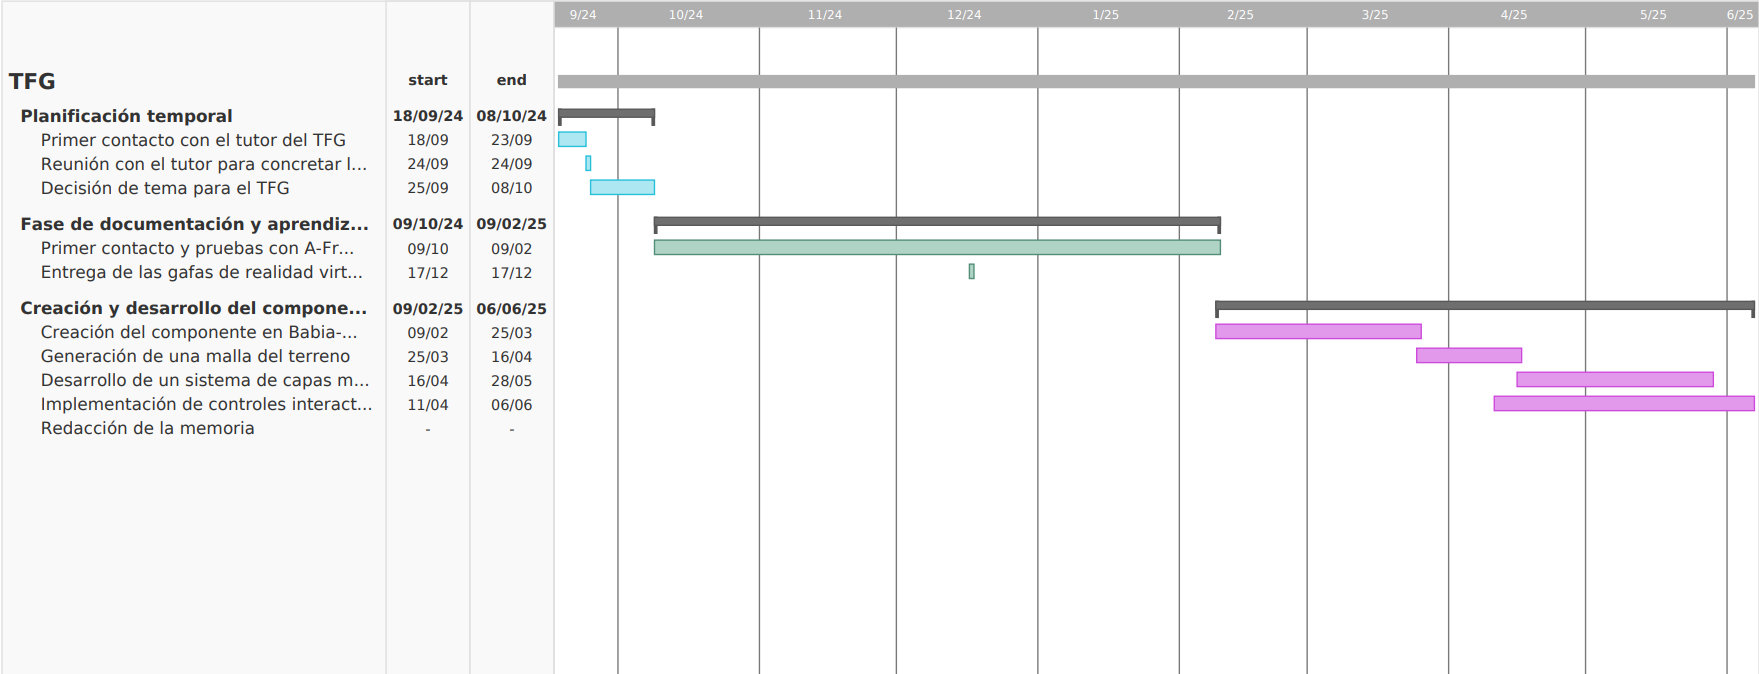
\includegraphics[width=\textwidth]{img/gantt.png}
  \caption{Diagrama de Gantt del TFG.}
  \label{fig:gantt}
\end{figure}

%%%%%%%%%%%%%%%%%%%%%%%%%%%%%%%%%%%%%%%%%%%%%%%%%%%%%%%%%%%%%%%%%%%%%%%%%%%%%%%%
%%%%%%%%%%%%%%%%%%%%%%%%%%%%%%%%%%%%%%%%%%%%%%%%%%%%%%%%%%%%%%%%%%%%%%%%%%%%%%%%
% ESTADO DEL ARTE %
%%%%%%%%%%%%%%%%%%%%%%%%%%%%%%%%%%%%%%%%%%%%%%%%%%%%%%%%%%%%%%%%%%%%%%%%%%%%%%%%

\cleardoublepage
\chapter{Estado del arte}
\label{chap:estado}

% Descripción de las tecnologías que utilizas en tu trabajo. 
% Con dos o tres párrafos por cada tecnología, vale. 
% Se supone que aquí viene todo lo que no has hecho tú.

% Puedes citar libros, como el de Bonabeau et al., sobre procesos estigmérgicos~\cite{bonabeau:_swarm}. 
% Me encantan los procesos estigmérgicos.
% Deberías leer más sobre ellos.
% Pero quizás no ahora, que tenemos que terminar la memoria para sacarnos por fin el título.
% Nota que el \~ \ añade un espacio en blanco, pero no deja que exista un salto de línea. 
% Imprescindible ponerlo para las citas.

% Citar es importantísimo en textos científico-técnicos. 
% Porque no partimos de cero.
% Es más, partir de cero es de tontos; lo suyo es aprovecharse de lo ya existente para construir encima y hacer cosas más sofisticadas.
% ¿Dónde puedo encontrar textos científicos que referenciar?
% Un buen sitio es Google Scholar\footnote{\url{http://scholar.google.com}}.
% Por ejemplo, si buscas por ``stigmergy libre software'' para encontrar trabajo sobre software libre y el concepto de \emph{estigmergia} (¿te he comentado que me gusta el concepto de estigmergia ya?), encontrarás un artículo que escribí hace tiempo cuyo título es ``Self-organized development in libre software: a model based on the stigmergy concept''.
% Si pulsas sobre las comillas dobles (entre la estrella y el ``citado por ...'', justo debajo del extracto del resumen del artículo, te saldrá una ventana emergente con cómo citar.
% Abajo a la derecha, aparece un enlace BibTeX.
% Púlsalo y encontrarás la referencia en formato BibTeX, tal que así:

% {\footnotesize
% \begin{verbatim}
% @inproceedings{robles2005self,
%   title={Self-organized development in libre software:
%          a model based on the stigmergy concept},
%   author={Robles, Gregorio and Merelo, Juan Juli\'an 
%           and Gonz\'alez-Barahona, Jes\'us M.},
%   booktitle={ProSim'05},
%   year={2005}
% }
% \end{verbatim}
% }

% Copia el texto en BibTeX y pégalo en el fichero \texttt{memoria.bib}, que es donde están las referencias bibliográficas.
% Para incluir la referencia en el texto de la memoria, deberás citarlo, como hemos hecho antes con~\cite{bonabeau:_swarm}, lo que pasa es que en vez de el identificador de la cita anterior (bonabeau:\_swarm), tendrás que poner el nuevo (robles2005self).
% Compila el fichero \texttt{memoria.tex} (\texttt{pdflatex memoria.tex}), añade la bibliografía (\texttt{bibtex memoria.aux}) y vuelve a compilar \texttt{memoria.tex} (\texttt{pdflatex memoria.tex})\ldots y \emph{voilà} ¡tenemos una nueva cita~\cite{robles2005self}!

% También existe la posibilidad de poner notas al pie de página, por ejemplo, una para indicarte que visite la página del GSyC\footnote{\url{http://gsyc.es}}.

\section{Babia-XR}
\label{sec:babiaxr}

\textit{Babia XR} es una plataforma de desarrollo para entornos inmersivos y experiencias interactivas en realidad virtual (VR), realidad aumentada (AR) y realidad mixta (MR). Se trata de una iniciativa impulsada por investigadores y docentes de la Universidad Rey Juan Carlos (URJC), lo que refuerza su vinculación con el ámbito académico y su aplicación en proyectos de investigación y desarrollo tecnológico.

El objetivo principal de Babia XR es facilitar la creación de aplicaciones inmersivas mediante tecnologías web abiertas, como \textit{WebXR}, \textit{A-Frame} y \textit{Three.js}. Estas tecnologías permiten ejecutar contenidos tridimensionales directamente en navegadores compatibles, sin necesidad de instalar software adicional. Esto representa una ventaja significativa en términos de accesibilidad, portabilidad y compatibilidad con múltiples dispositivos, incluyendo gafas de realidad virtual como las Meta Quest.

En el contexto de este trabajo, Babia XR se utiliza como entorno base para la integración del componente de visualización de mapas tridimensionales. La elección de esta plataforma responde a dos motivos principales:

\begin{enumerate}
  \item \textbf{Necesidad técnica:} proporciona la infraestructura necesaria para desplegar escenas VR complejas, integrando capas de información geoespacial, controles de navegación y representaciones 3D sobre terrenos reales.
  \item \textbf{Vinculación institucional:} al tratarse de una herramienta desarrollada dentro de la propia universidad, su uso refuerza la colaboración entre estudiantes y líneas de investigación del centro, además de facilitar el acceso a soporte técnico y documentación específica.
\end{enumerate}

Babia XR se apoya en un conjunto de tecnologías modernas y bien consolidadas:
\begin{itemize}
  \item \textit{A-Frame}: framework basado en HTML para crear experiencias VR accesibles desde navegadores.
  \item \textit{Three.js}: biblioteca JavaScript que permite renderizar gráficos 3D en WebGL con gran flexibilidad.
  \item \textit{WebXR}: estándar para ejecutar experiencias inmersivas directamente en el navegador, compatible con múltiples dispositivos.
\end{itemize}

Gracias a esta combinación, Babia XR permite un desarrollo ágil y modular, facilitando la incorporación de componentes personalizados, como el sistema de teselas con desplazamiento que se ha implementado en este proyecto.


\subsection{A-Frame}
\label{subsec:aframe}

\textit{A-Frame} es un framework de código abierto desarrollado inicialmente por Mozilla para facilitar la creación de experiencias de realidad virtual usando HTML. Su diseño declarativo permite definir escenas tridimensionales mediante etiquetas similares a las del propio lenguaje HTML, lo cual lo hace accesible incluso para desarrolladores con conocimientos limitados de gráficos 3D o WebGL.

\textit{A-Frame} está construido sobre \texttt{Three.js}, lo que le permite mantener una gran potencia gráfica bajo una capa de abstracción más sencilla. Además, es extensible mediante componentes personalizados, lo que permite adaptar el comportamiento de los elementos de la escena a las necesidades específicas del proyecto.

En este trabajo, \textit{A-Frame} actúa como base para representar los elementos visuales del mapa tridimensional, así como para integrar los controles de usuario, cámaras, luces y otros objetos interactivos.

\begin{figure}[H]
  \centering
  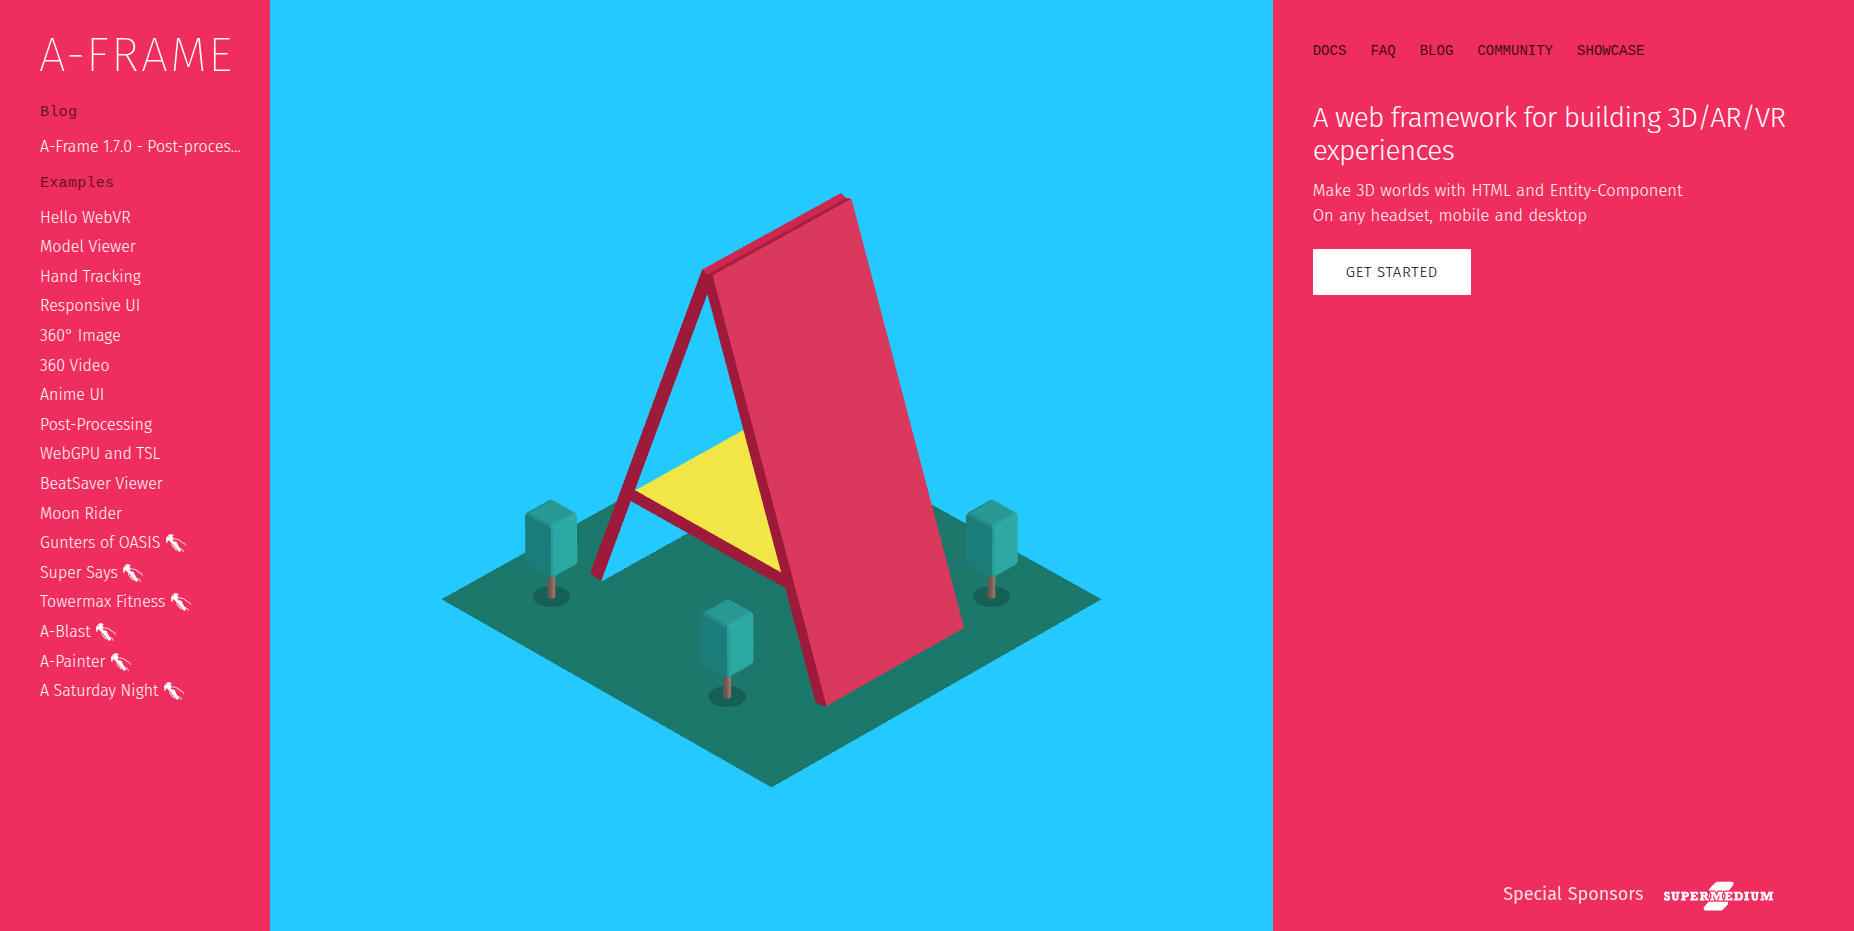
\includegraphics[width=\textwidth]{img/aframe.png}
  \caption{Sitio web oficial de \textit{A-Frame}.}
  \label{fig:aframe-img}
\end{figure}


\subsection{Three.js}
\label{subsec:threejs}

Three.js es una biblioteca JavaScript muy utilizada para renderizar gráficos tridimensionales en el navegador utilizando \texttt{WebGL}. Proporciona una interfaz de alto nivel que simplifica el uso de funcionalidades avanzadas de gráficos 3D, como luces dinámicas, materiales complejos, sombras en tiempo real y animaciones.

En el contexto de Babia XR, Three.js es el motor gráfico que subyace bajo \textit{A-Frame}. Aunque normalmente no se accede directamente a su API cuando se utiliza \textit{A-Frame}, su presencia es fundamental para permitir el renderizado eficiente de los objetos en la escena.

Algunos componentes personalizados del proyecto, especialmente los relacionados con el desplazamiento de texturas y la carga dinámica de teselas, se benefician de las capacidades avanzadas de Three.js, ya que permiten modificar directamente atributos de materiales y geometrías a bajo nivel.

\subsubsection*{WebGL}
\label{subsec:webgl}

WebGL (Web Graphics Library) es una API de JavaScript para renderizar gráficos 2D y 3D dentro de cualquier navegador web compatible sin necesidad de plugins. Está basada en OpenGL ES 2.0 y permite acceder a la aceleración gráfica del hardware de forma segura. En el contexto del proyecto, WebGL es la tecnología subyacente sobre la que se construyen bibliotecas como Three.js y A-Frame, lo que permite representar escenas tridimensionales complejas directamente en el navegador.


\subsection{WebXR}
\label{subsec:webxr}

WebXR es un estándar del W3C que proporciona una interfaz unificada para acceder a dispositivos de realidad virtual y aumentada desde navegadores web. Permite detectar dispositivos compatibles (como gafas VR o móviles con capacidades AR), obtener sus posiciones y orientaciones en tiempo real, y renderizar escenas de forma inmersiva.

A diferencia de sus predecesores (como WebVR), WebXR está diseñado para soportar tanto realidad virtual como aumentada desde una misma API, y su adopción por parte de los principales navegadores modernos garantiza su viabilidad a largo plazo.

Babia XR utiliza WebXR para habilitar la ejecución de escenas inmersivas en dispositivos como las Meta Quest, permitiendo al usuario entrar en la experiencia VR directamente desde el navegador. Esta capacidad resulta especialmente útil en entornos educativos y de investigación, donde la simplicidad de despliegue es una prioridad.


\section{HTML}
\label{sec:html}

HTML (\textit{HyperText Markup Language}) es el lenguaje estándar para estructurar contenido en la web. En este proyecto, HTML se emplea como base para organizar y enlazar los elementos visuales de la interfaz del componente, además de ser fundamental para la integración de \textit{A-Frame}, que utiliza etiquetas personalizadas dentro de documentos HTML para definir entidades 3D y escenas interactivas.

\begin{figure}[H]
  \centering
  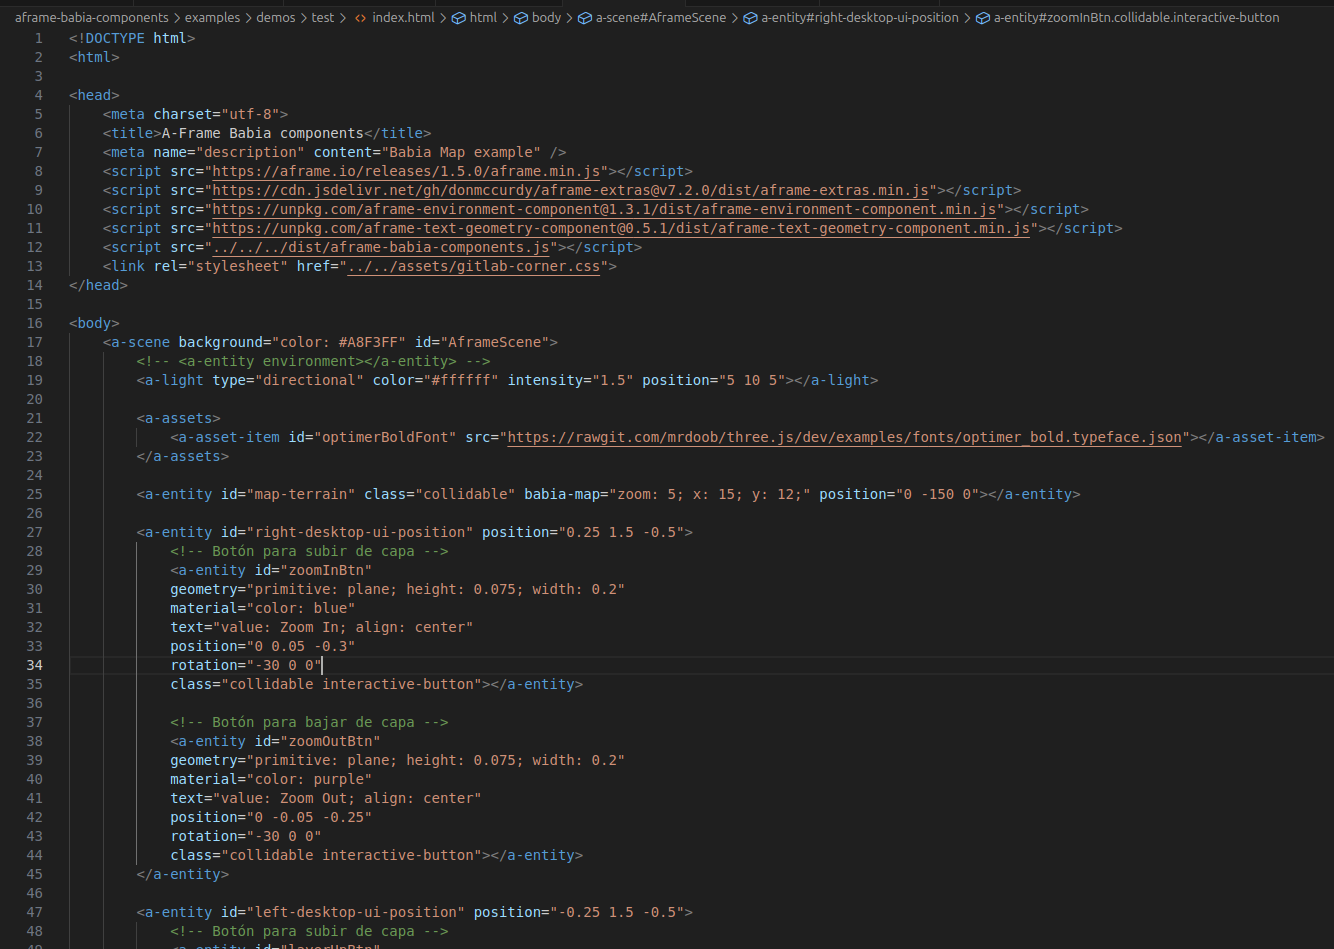
\includegraphics[width=\textwidth]{img/html.png}
  \caption{Código HTML del componente.}
  \label{fig:html-img}
\end{figure}



\section{JavaScript y Node.js}
\label{sec:js-node}

JavaScript es el lenguaje de programación principal del entorno web, y se utiliza tanto en el desarrollo de interfaces interactivas como en la lógica del componente desarrollado. Permite manipular elementos HTML, responder a eventos del usuario y controlar el comportamiento del componente en tiempo real.

\begin{figure}[H]
  \centering
  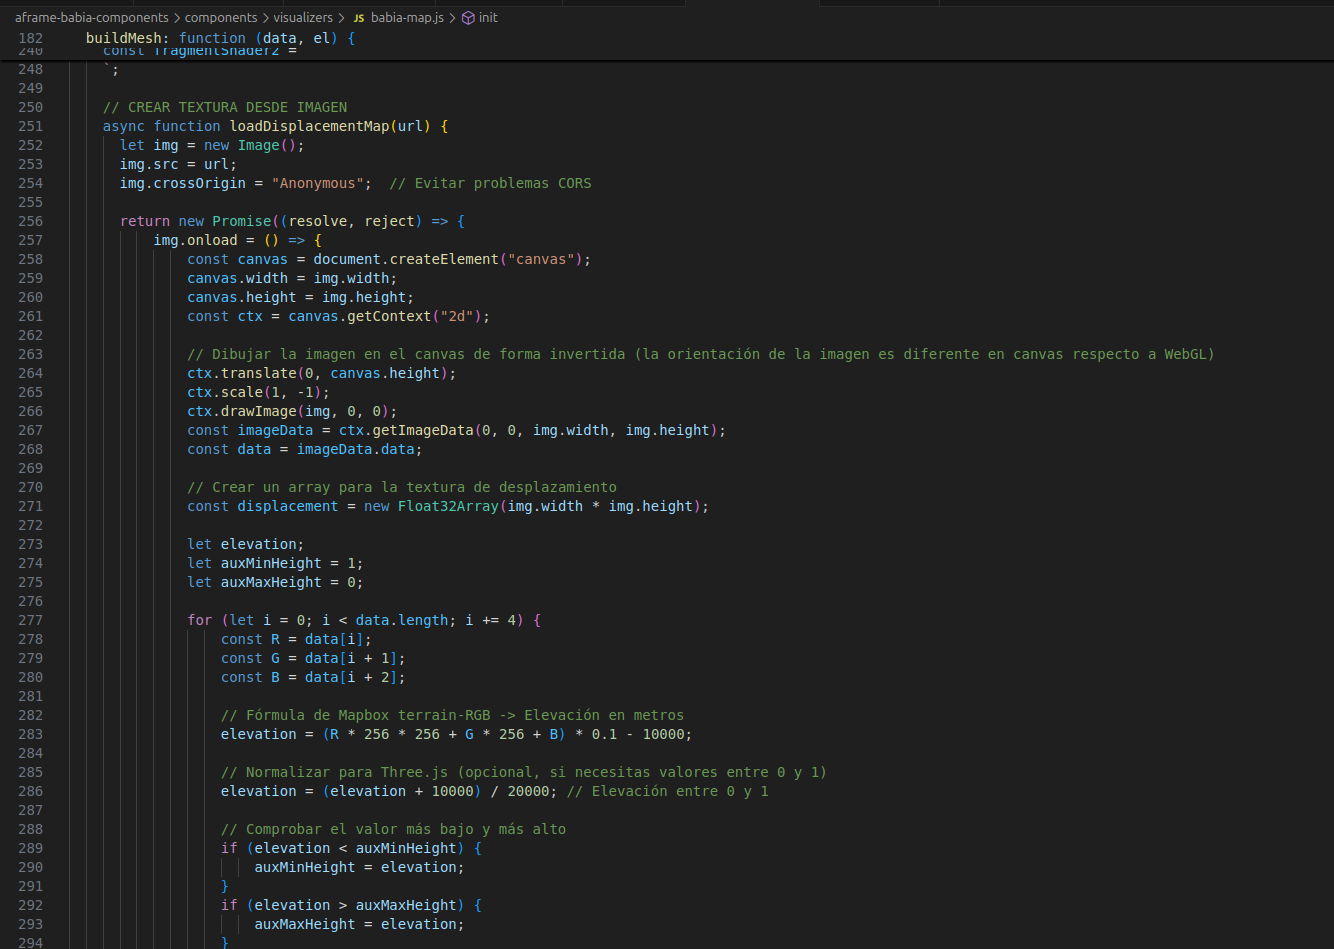
\includegraphics[width=\textwidth]{img/js.png}
  \caption{Código fuente en \textit{JavaScript} del componente.}
  \label{fig:js-img}
\end{figure}


\subsection{Node.js y herramientas asociadas}
\label{sec:nodejs}

Node.js es un entorno de ejecución para JavaScript fuera del navegador. Aunque el componente se ejecuta en el cliente, Node.js se utiliza durante el desarrollo para gestionar dependencias, ejecutar scripts y automatizar tareas. Para ello, se hace uso de \texttt{npm} (Node Package Manager), el gestor de paquetes de Node.js, y de \texttt{nvm} (Node Version Manager), que facilita la instalación y gestión de múltiples versiones de Node.js en un mismo sistema. Estas herramientas son necesarias para compilar, organizar y desplegar el componente de manera eficiente.



\section{APIs de Mapbox y \textit{OpenStreetMap}}
\label{sec:apis}

Mapbox y \textit{OpenStreetMap} son servicios que proporcionan datos cartográficos. \textit{OpenStreetMap} (OSM) es una iniciativa colaborativa que ofrece mapas del mundo creados por una comunidad de voluntarios. Por su parte, Mapbox utiliza datos de OSM y otras fuentes para ofrecer un conjunto de APIs avanzadas orientadas al desarrollo web, como mapas personalizados, capas de estilo y servicios de geolocalización.

En este proyecto se hace uso de estas APIs para obtener datos de elevación y estilos visuales (como capas satelitales o vistas de calle) que se aplican sobre la malla del terreno generada en el componente. Mapbox requiere un \textit{token} de acceso personal, mientras que OSM puede utilizarse directamente mediante peticiones a sus servidores abiertos.

\begin{figure}[H]
  \centering
  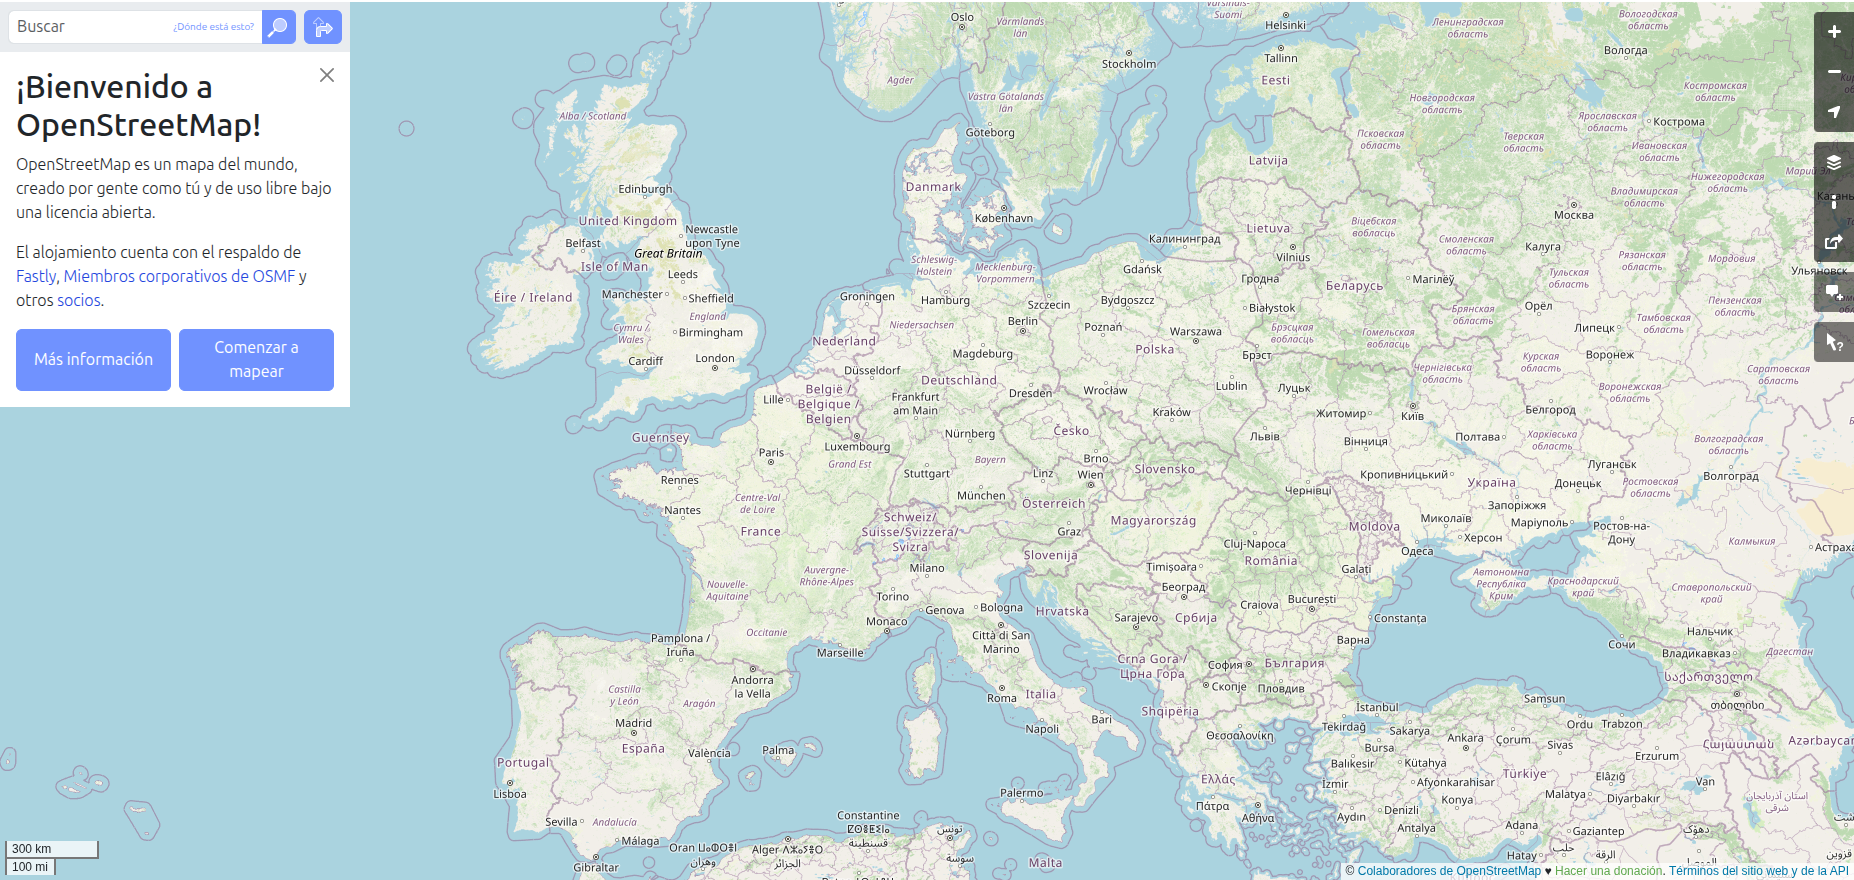
\includegraphics[width=\textwidth]{img/osm.png}
  \caption{Sitio web oficial de \textit{OpenStreetMap}.}
  \label{fig:osm}
\end{figure}



\section{Gafas de Realidad Virtual: Meta Quest 3}
\label{sec:gafas}

Las Meta Quest 3, desarrolladas por Meta (anteriormente Oculus), son unas gafas de realidad virtual autónomas que permiten ejecutar aplicaciones VR sin necesidad de un ordenador externo. Disponen de controladores hápticos, sensores de movimiento y capacidad de realidad mixta (passthrough a color), lo que las convierte en una herramienta ideal para pruebas e implementación de experiencias inmersivas.

Gracias al soporte de WebXR en su navegador interno, estas gafas permiten ejecutar el componente desarrollado directamente desde la web, lo que facilita el proceso de validación en un entorno real.

\begin{figure}[H]
  \centering
  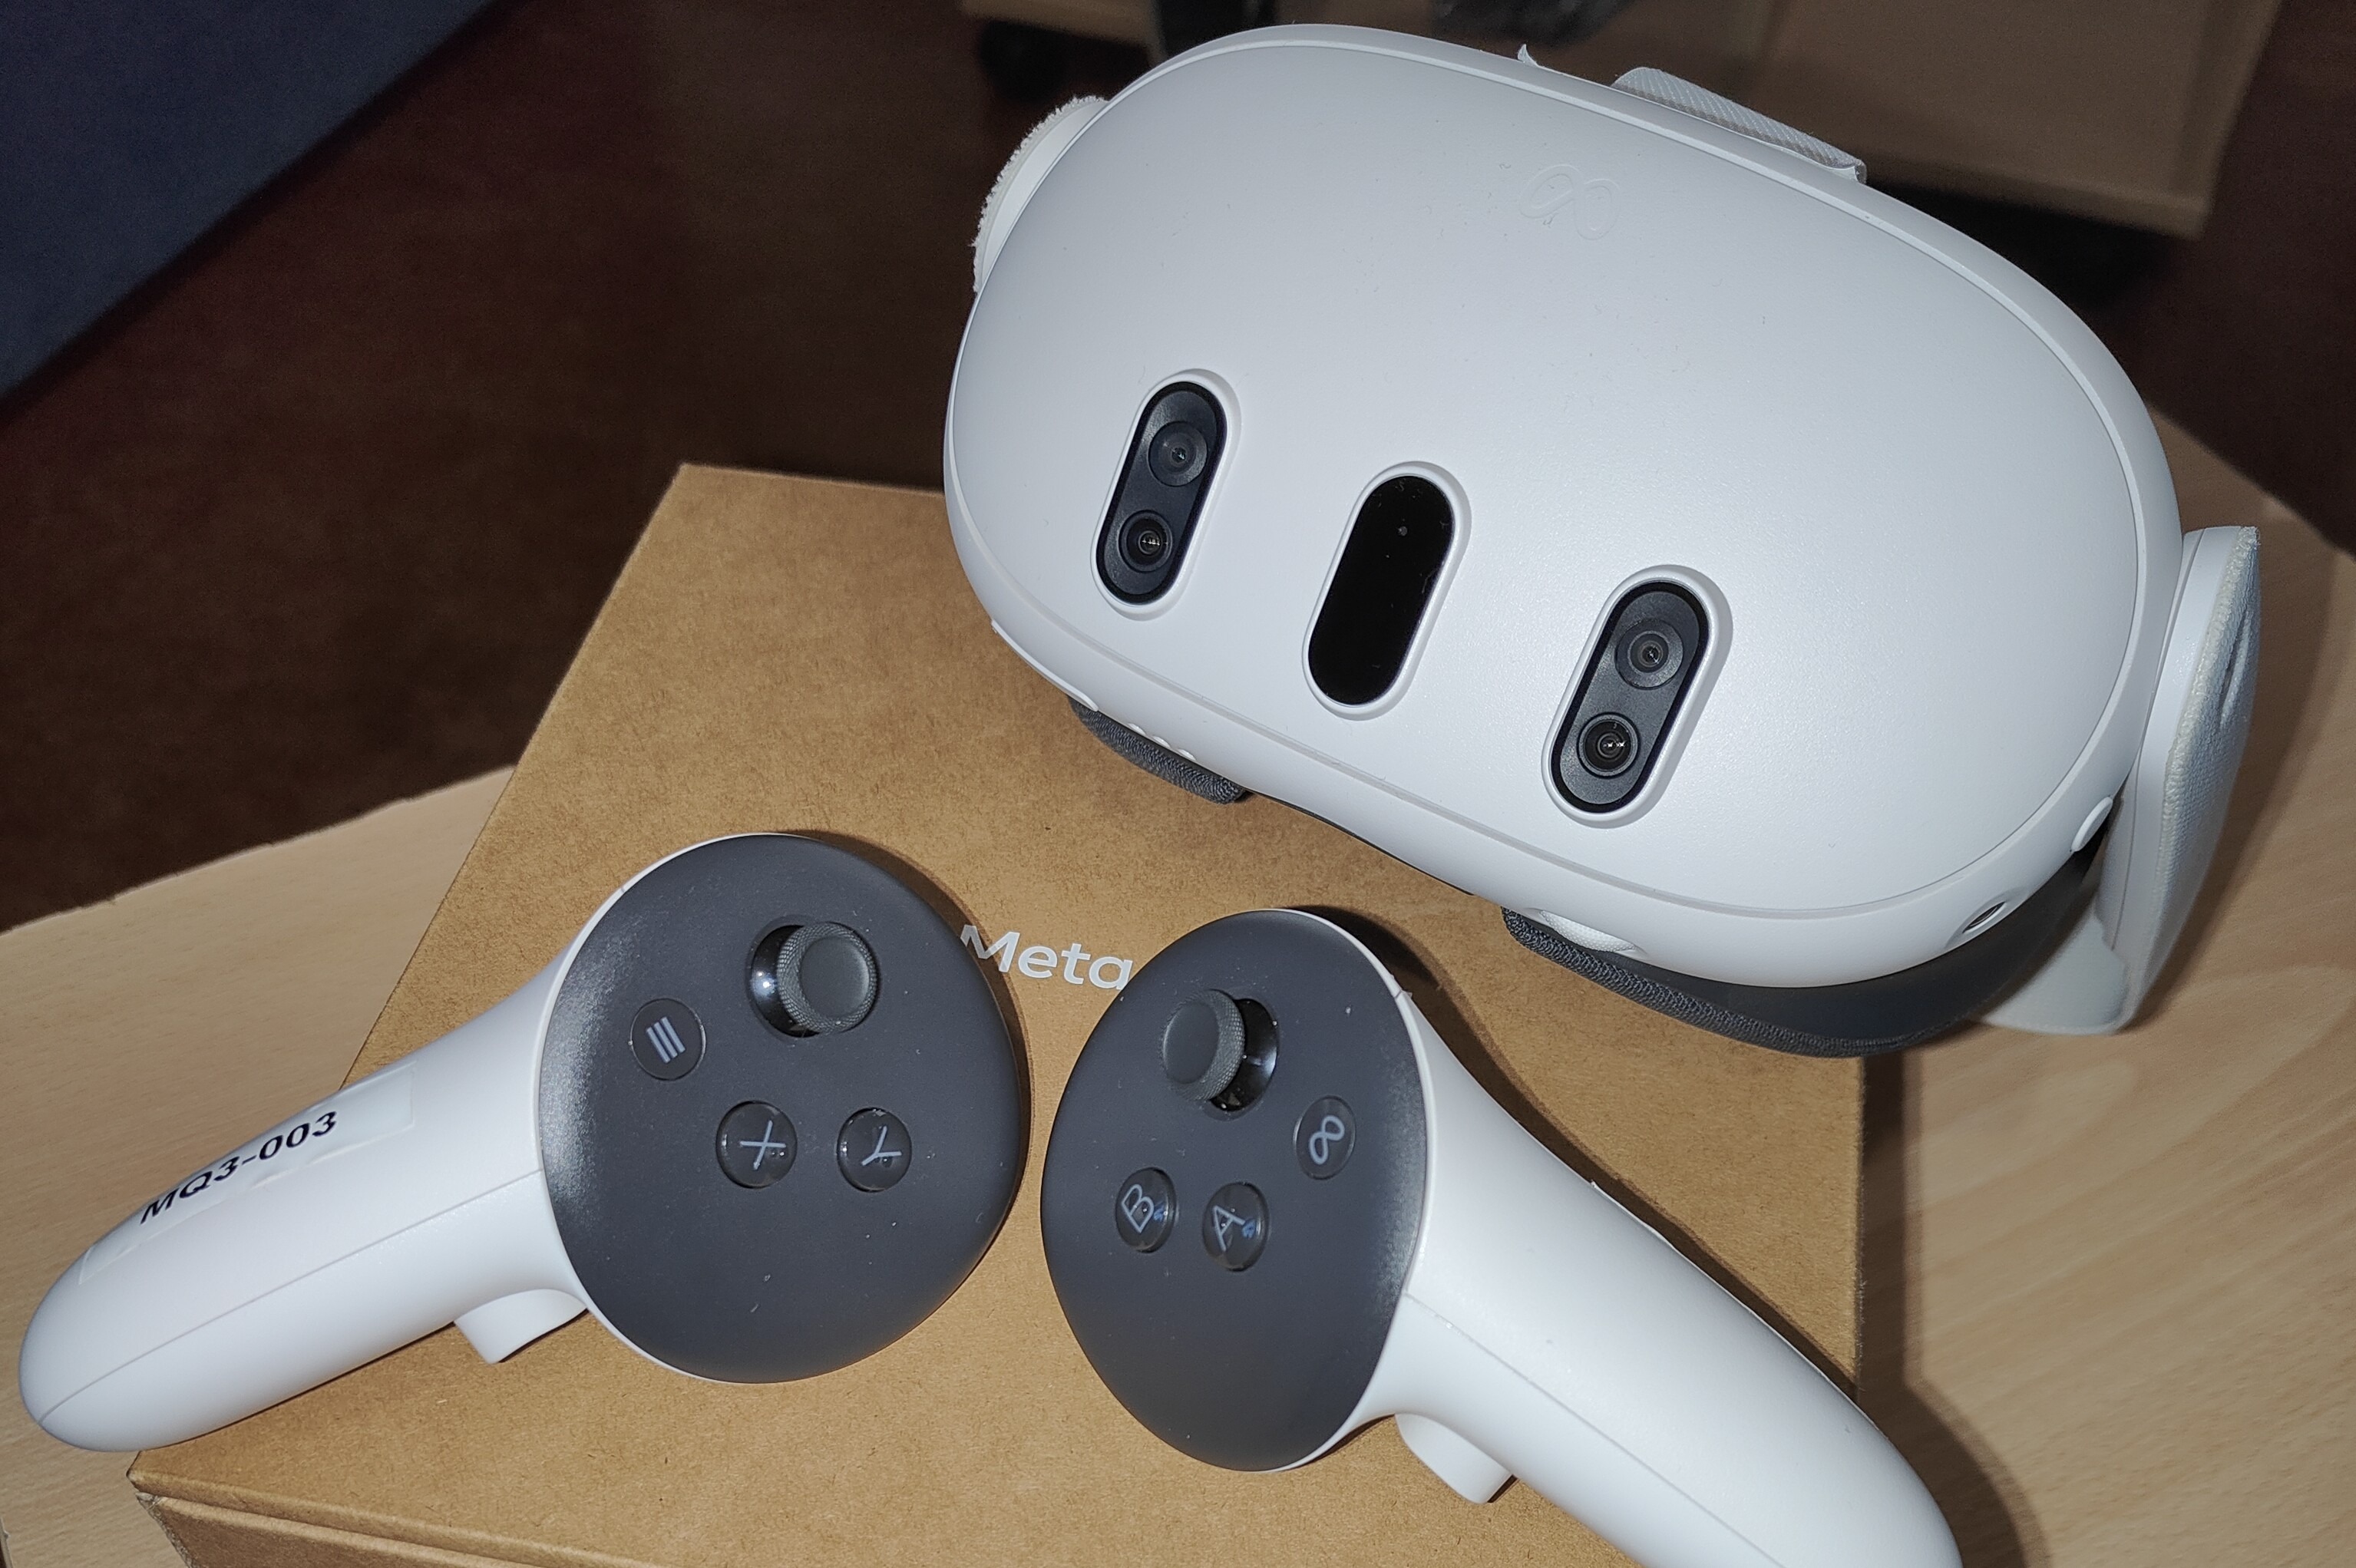
\includegraphics[width=\textwidth]{img/gafas.jpg}
  \caption{Gafas prestadas por la universidad.}
  \label{fig:osm}
\end{figure}



\section{Editor de Código: Visual Studio Code}
\label{sec:vscode}

Visual Studio Code (VS Code) es un editor de código fuente desarrollado por Microsoft, ampliamente adoptado por la comunidad de desarrolladores. Ofrece integración con sistemas de control de versiones, depuración, resaltado de sintaxis y soporte para extensiones que facilitan el desarrollo web y VR.

Durante el desarrollo del proyecto, se ha utilizado como entorno principal de trabajo, aprovechando su integración con herramientas como Git, su terminal integrada para la ejecución de comandos Node.js y su compatibilidad con tecnologías web modernas.



\section{Apoyo de herramientas de inteligencia artificial}
\label{sec:ias}

Durante el desarrollo del proyecto, se ha contado con el apoyo de herramientas basadas en inteligencia artificial como ChatGPT, que han sido útiles para resolver dudas técnicas, refinar la redacción de la documentación, generar fragmentos de código y comprender tecnologías específicas de forma más ágil.

Estas herramientas, si bien no sustituyen el conocimiento técnico, han servido como soporte complementario para acelerar el proceso de desarrollo, ahorrar tiempo en tareas repetitivas y mejorar la calidad de la documentación generada.


% \section{Sección 1} 
% \label{sec:seccion1}

% Hemos hablado de cómo incluir figuras.
% Pero no hemos dicho nada de tablas.
% A mí me gustan las tablas.
% Mucho.
% Aquí un ejemplo de tabla, la Tabla~\ref{tab:ejemplo} (siento ser pesado, pero nota cómo he puesto la referencia).

% \begin{table}
%  \begin{center}
%   \begin{tabular}{ | l | c | r |} % tenemos tres colummnas, la primera alineada a la izquierda (l), la segunda al centro (c) y la tercera a la derecha (r). El | indica que entre las columnas habrá una línea separadora.
%     \hline
%     Uno & 2 & 3 \\ \hline % el hline nos da una línea vertical
%     Cuatro & 5 & 6 \\ \hline
%     Siete & 8 & 9 \\
%     \hline
%   \end{tabular}
%   \caption{Ejemplo de tabla. Aquí viene una pequeña descripción (el \emph{caption}, el pie de tabla/figura) del contenido de la tabla. Si la tabla no es autoexplicativa, siempre viene bien aclararla aquí.}
%   \label{tab:ejemplo}
%  \end{center}
% \end{table}

% Hay un sitio en Internet donde puedes diseñar las tablas fácilmente y luego hacer un corta y pega del resultado en tu editor.
% Puedes probarlo en \url{https://www.tablesgenerator.com/}.



%%%%%%%%%%%%%%%%%%%%%%%%%%%%%%%%%%%%%%%%%%%%%%%%%%%%%%%%%%%%%%%%%%%%%%%%%%%%%%%%
%%%%%%%%%%%%%%%%%%%%%%%%%%%%%%%%%%%%%%%%%%%%%%%%%%%%%%%%%%%%%%%%%%%%%%%%%%%%%%%%
% DISEÑO E IMPLEMENTACIÓN %
%%%%%%%%%%%%%%%%%%%%%%%%%%%%%%%%%%%%%%%%%%%%%%%%%%%%%%%%%%%%%%%%%%%%%%%%%%%%%%%%

\cleardoublepage
\chapter{Diseño e implementación}
\label{sec:diseno}

Aquí viene todo lo que has hecho tú (tecnológicamente). 
Puedes entrar hasta el detalle. 
Es la parte más importante de la memoria, porque describe lo que has hecho tú.
Eso sí, normalmente aconsejo no poner código, sino diagramas.



\section{Arquitectura general} 
\label{sec:arquitectura}

Si tu proyecto es un software, siempre es bueno poner la arquitectura (que es cómo se estructura tu programa a ``vista de pájaro'').

\begin{figure}
  \centering
  \includegraphics[width=9cm, keepaspectratio]{img/arquitectura.png}
  \caption{Estructura del parser básico}
  \label{fig:arquitectura}
\end{figure}


Por ejemplo, puedes verlo en la figura~\ref{fig:arquitectura}.
\LaTeX \ pone las figuras donde mejor cuadran. 
Y eso quiere decir que quizás no lo haga donde lo hemos puesto\ldots 
Eso no es malo.
A veces queda un poco raro, pero es la filosofía de \LaTeX: tú al contenido, que yo me encargo de la maquetación.


 
Recuerda que toda figura que añadas a tu memoria debe ser explicada.
Sí, aunque te parezca evidente lo que se ve en la figura~\ref{fig:arquitectura}, la figura en sí solamente es un apoyo a tu texto.
Así que explica lo que se ve en la figura, haciendo referencia a la misma tal y como ves aquí.
Por ejemplo: En la figura~\ref{fig:arquitectura} se puede ver que la estructura del \emph{parser} básico, que consta de seis componentes diferentes: los datos se obtienen de la red, y según el tipo de dato, se pasará a un \emph{parser} específico y bla, bla, bla\ldots

Si utilizas una base de datos, no te olvides de incluir también un diagrama de entidad-relación.


%%%%%%%%%%%%%%%%%%%%%%%%%%%%%%%%%%%%%%%%%%%%%%%%%%%%%%%%%%%%%%%%%%%%%%%%%%%%%%%%
%%%%%%%%%%%%%%%%%%%%%%%%%%%%%%%%%%%%%%%%%%%%%%%%%%%%%%%%%%%%%%%%%%%%%%%%%%%%%%%%
% EXPERIMENTOS Y VALIDACIÓN %
%%%%%%%%%%%%%%%%%%%%%%%%%%%%%%%%%%%%%%%%%%%%%%%%%%%%%%%%%%%%%%%%%%%%%%%%%%%%%%%%

\cleardoublepage
\chapter{Experimentos y validación}
\label{chap:experimentos}

Este capítulo se introdujo como requisito en 2019. 
Describe los experimentos y casos de test que tuviste que implementar para validar tus resultados. 
Incluye también los resultados de validación que permiten afirmar que tus resultados son correctos. 


%%%%%%%%%%%%%%%%%%%%%%%%%%%%%%%%%%%%%%%%%%%%%%%%%%%%%%%%%%%%%%%%%%%%%%%%%%%%%%%%
%%%%%%%%%%%%%%%%%%%%%%%%%%%%%%%%%%%%%%%%%%%%%%%%%%%%%%%%%%%%%%%%%%%%%%%%%%%%%%%%
% RESULTADOS %
%%%%%%%%%%%%%%%%%%%%%%%%%%%%%%%%%%%%%%%%%%%%%%%%%%%%%%%%%%%%%%%%%%%%%%%%%%%%%%%%

\cleardoublepage
\chapter{Resultados}
\label{chap:resultados}

En este capítulo se incluyen los resultados de tu trabajo fin de grado.

Si es una herramienta de análisis lo que has realizado, aquí puedes poner ejemplos de haberla utilizado para que se vea su utilidad.


%%%%%%%%%%%%%%%%%%%%%%%%%%%%%%%%%%%%%%%%%%%%%%%%%%%%%%%%%%%%%%%%%%%%%%%%%%%%%%%%
%%%%%%%%%%%%%%%%%%%%%%%%%%%%%%%%%%%%%%%%%%%%%%%%%%%%%%%%%%%%%%%%%%%%%%%%%%%%%%%%
% CONCLUSIONES %
%%%%%%%%%%%%%%%%%%%%%%%%%%%%%%%%%%%%%%%%%%%%%%%%%%%%%%%%%%%%%%%%%%%%%%%%%%%%%%%%

\cleardoublepage
\chapter{Conclusiones}
\label{chap:conclusiones}


\section{Consecución de objetivos}
\label{sec:consecucion-objetivos}

Esta sección es la sección espejo de las dos primeras del capítulo de objetivos, donde se planteaba el objetivo general y se elaboraban los específicos.

Es aquí donde hay que debatir qué se ha conseguido y qué no. 
Cuando algo no se ha conseguido, se ha de justificar, en términos de qué problemas se han encontrado y qué medidas se han tomado para mitigar esos problemas.

Y si has llegado hasta aquí, siempre es bueno pasarle el corrector ortográfico, que las erratas quedan fatal en la memoria final.
Para eso, en Linux tenemos aspell, que se ejecuta de la siguiente manera desde la línea de \emph{shell}:

\begin{verbatim}
  aspell --lang=es_ES -c memoria.tex
\end{verbatim}

\section{Aplicación de lo aprendido}
\label{sec:aplicacion}

Aquí viene lo que has aprendido durante el Grado/Máster y que has aplicado en el TFG/TFM.
Una buena idea es poner las asignaturas más relacionadas y comentar en un párrafo los conocimientos y habilidades puestos en práctica.

\begin{enumerate}
  \item a
  \item b
\end{enumerate}


\section{Lecciones aprendidas}
\label{sec:lecciones_aprendidas}

Aquí viene lo que has aprendido en el Trabajo Fin de Grado/Máster.

\begin{enumerate}
  \item Aquí viene uno.
  \item Aquí viene otro.
\end{enumerate}


\section{Trabajos futuros}
\label{sec:trabajos_futuros}

Ningún proyecto ni software se termina, así que aquí vienen ideas y funcionalidades que estaría bien tener implementadas en el futuro.

Es un apartado que sirve para dar ideas de cara a futuros TFGs/TFMs.


%%%%%%%%%%%%%%%%%%%%%%%%%%%%%%%%%%%%%%%%%%%%%%%%%%%%%%%%%%%%%%%%%%%%%%%%%%%%%%%%
%%%%%%%%%%%%%%%%%%%%%%%%%%%%%%%%%%%%%%%%%%%%%%%%%%%%%%%%%%%%%%%%%%%%%%%%%%%%%%%%
% APÉNDICE(S) %
%%%%%%%%%%%%%%%%%%%%%%%%%%%%%%%%%%%%%%%%%%%%%%%%%%%%%%%%%%%%%%%%%%%%%%%%%%%%%%%%

\cleardoublepage
\appendix
\chapter{Manual de usuario}
\label{app:manual}

Esto es un apéndice.
Si has creado una aplicación, siempre viene bien tener un manual de usuario.
Pues ponlo aquí.

%%%%%%%%%%%%%%%%%%%%%%%%%%%%%%%%%%%%%%%%%%%%%%%%%%%%%%%%%%%%%%%%%%%%%%%%%%%%%%%%
%%%%%%%%%%%%%%%%%%%%%%%%%%%%%%%%%%%%%%%%%%%%%%%%%%%%%%%%%%%%%%%%%%%%%%%%%%%%%%%%
% BIBLIOGRAFIA %
%%%%%%%%%%%%%%%%%%%%%%%%%%%%%%%%%%%%%%%%%%%%%%%%%%%%%%%%%%%%%%%%%%%%%%%%%%%%%%%%

\cleardoublepage

% Las siguientes dos instrucciones es todo lo que necesitas
% para incluir las citas en la memoria
\bibliographystyle{abbrv}
\bibliography{memoria}  % memoria.bib es el nombre del fichero que contiene
% las referencias bibliográficas. Abre ese fichero y mira el formato que tiene,
% que se conoce como BibTeX. Hay muchos sitios que exportan referencias en
% formato BibTeX. Prueba a buscar en http://scholar.google.com por referencias
% y verás que lo puedes hacer de manera sencilla.
% Más información: 
% http://texblog.org/2014/04/22/using-google-scholar-to-download-bibtex-citations/

\end{document}
